\documentclass[10pt]{article}
\usepackage[margin=1.7cm]{geometry}
\usepackage{multicol}
\usepackage{amsmath, amssymb}
\usepackage{graphicx}
\usepackage{tikz}
\usepackage{pgfplots}
\pgfplotsset{compat=1.18}
\usepackage{xcolor}
\usepackage{booktabs}
\usepackage{enumitem}
\usepackage[hidelinks]{hyperref}
\usepackage{titlesec}
\usepackage{caption}
\usepackage{float}
\usepackage[round,authoryear]{natbib}

% Inline figure environment usable inside multicols (no floating).
\newenvironment{Figure}{\par\medskip\noindent\begin{minipage}{\linewidth}\centering}
                       {\medskip\end{minipage}\par\medskip}

\titleformat{\section}{\large\bfseries}{\thesection}{0.8em}{}
\titleformat{\subsection}{\normalsize\bfseries}{\thesubsection}{0.6em}{}
\setlength{\columnsep}{0.7cm}

% colours
\definecolor{epi}{HTML}{2A7F8C}
\definecolor{val}{HTML}{B5651D}
\definecolor{re}{HTML}{6B3FA0}
\definecolor{mcmc}{HTML}{888888}
\definecolor{nsga}{HTML}{D43F3A}
\definecolor{onepass}{HTML}{4C9F38}

\title{\bfseries Moral Reasoning on the Pareto Frontier\\
\normalsize\itshape A multi-objective view of epistemic and ethical values, and why equilibrium-style methods are well-suited to traverse it}
\author{}
\date{\small Draft, \today}

\begin{document}
\maketitle

\begin{abstract}\small
\noindent
What counts as good moral reasoning when there is no single ground truth?
We propose a multi-objective view in which a moral position --- a set of
commitments together with a set of principles that account for them --- is
evaluated against two axis families that genuinely conflict. The primary axes
are \emph{ethical}: principles carry fuzzy loadings on moral values, and we
work with five --- \textsc{freedom}, \textsc{solidarity}, \textsc{justice},
\textsc{welfare}, and \textsc{dignity} --- chosen so that the central
tensions of moral life (liberty vs.\ community, fairness vs.\ welfare,
welfare vs.\ dignity) appear directly as trade-offs among axes. The secondary
axes are \emph{epistemic} measures of internal coherence, drawn from the formal
account of \citet{beisbart2021}: account, systematicity, and faithfulness.
Every reachable position occupies a point in this joint space, and the
rational object of study is its \emph{Pareto frontier}: the set of attainable
positions for which no other position is at least as good on every axis and
strictly better on at least one. We argue that this reframes the central
question of moral reasoning from ``which position is right?'' to ``which
strategy reliably finds positions on the frontier?''~--- and that the question
favours \emph{equilibrium-style methods} that balance competing values, because
without a ground truth the best a reasoner can do is settle on a defensible
middle. We sketch a pilot using MoReBench dilemmas and an LLM-based reasoning
system we have already prototyped.
\end{abstract}

\begin{multicols}{2}

\section{Motivation: moral reasoning without a ground truth}

Moral reasoning has long resisted the model of justification that works elsewhere
in epistemology. There is no external fact of the matter that a moral position
\emph{tracks} the way an empirical belief tracks the world. Two careful reasoners
working from different starting intuitions can both reason responsibly and reach
different conclusions, and we do not, on reflection, want to say one of them is
just wrong --- pluralism in moral epistemology is widely accepted
\citep{elgin1996, rechnitzer2022}. The natural question, then, is not which
position is correct but \emph{what counts as good reasoning} in a domain where
the standard correctness criterion does not apply.

We argue that this question has a structural answer: good moral reasoning is
\emph{multi-objective}. A moral position is graded on at least two distinct
axis families. The primary ones are \emph{ethical}: a position carries weight
on different moral values --- freedom, solidarity, justice, welfare, dignity ---
and these values genuinely conflict. A position that maximises welfare may
underweight freedom; a position centred on dignity may not maximise welfare;
a position that elevates solidarity may sit uneasily with strong protections of
individual freedom. The choice of how to balance such tensions is what moral
reasoning is for.

In parallel, a position is graded \emph{epistemically} on how well it hangs
together as reasoning --- the principles should account for the commitments,
the principles should be compact and unifying, and the commitments should not
stray too far from the agent's starting intuitions. A formal account of these
coherence properties is available \citep{beisbart2021}. We take these as
secondary objectives: a morally interesting position that is internally
incoherent is not a serious candidate, but a perfectly coherent position can
still occupy any number of places in value-space, and the central
philosophical interest is in the latter.

When objectives genuinely conflict, the rational object of study is not a single
optimum but a \emph{Pareto frontier}: the set of attainable positions for which
no other position is at least as good on every objective and strictly better on
at least one. We claim that this is the right object of study for moral
reasoning, and that it gives us a new way to evaluate reasoning strategies. A
good strategy is one that reliably finds Pareto-optimal positions --- and
ideally finds interior (mixed) ones, since corner solutions (``maximise welfare
and nothing else'') are easy and uninteresting. We will argue that
\emph{equilibrium-style} methods --- methods that proceed by mutually adjusting
commitments and principles in light of each other --- are particularly
well-suited to this role, because they explicitly negotiate the kind of
trade-offs the frontier consists of. Reflective equilibrium, in this view, is
one instance of a broader family of equilibrium-style traversal strategies
worth studying empirically.

\section{The moral data resource}\label{sec:resource}

The methodological contribution we are pitching is a way to make moral
reasoning empirically studyable: construct a curated, mathematically defined
\emph{moral data resource}, then study reasoning strategies as pure traversal
algorithms on it. Three ideas combine.

\paragraph{Pre-enumerated inputs.} The candidates an agent might consider
when reasoning about the dataset --- specific case verdicts and candidate
moral principles --- are pre-enumerated. We construct a finite pool of
candidate commitments and a finite pool of candidate principles from a
dilemma source, then curate both pools with explicit quality control: fusion
of near-duplicates, deletion of weak candidates, per-principle scoring on
quality dimensions (independent systematicity, specificity, domain-fit), and
philosopher review of every retained candidate. The curated pool is intended
as a reusable resource in its own right, independent of any downstream
reasoning method.

\paragraph{Pre-enumerated inferential connections.} For every principle-%
commitment pair we pre-compute whether the principle entails the commitment,
contradicts it, or is silent on it. The result is a fixed, philosopher-%
validated inferential graph between principles and commitments.

\paragraph{Pre-tagged ethical values.} Each principle in the curated pool
carries a fuzzy value-loading vector distributing its weight across the five
values, also fixed during curation.

\paragraph{Reasoning becomes pure mathematics.} The combined output is a
fully specified moral space. \emph{Reasoning over it is then a purely
mathematical operation: a reasoning strategy is simply an algorithm that
selects, from the fixed pools, a subset of commitments and a subset of
principles subject to consistency, graded by the multi-objective evaluation
defined in Section~\ref{sec:formal}. No LLM participates in the reasoning
loop.} The LLM does its work during construction; all comparison of
strategies happens on a fixed substrate.

This decoupling is what makes the comparison cleanly interpretable. Current
debates about LLMs and moral reasoning conflate the \emph{moral content} a
model can articulate with the \emph{reasoning strategy} it employs. Here
those are separated: the moral content lives in the curated pool, validated
up-front; the strategies are pure mathematics operating on it.

\section{A formal model of the moral solution space}\label{sec:formal}

We adopt a formal model adapted from \citet{beisbart2021} and the simulation
infrastructure of \citet{freivogel2023}, extended with an explicit value layer.
We summarise the notation here and then state the multi-objective optimization
problem it gives rise to.

\paragraph{Pools.} Fix a finite pool of candidate moral commitments
$\mathcal{S}$ --- case verdicts indexed by the dilemmas in our dataset,
closed under negation --- a finite pool of candidate moral principles
$\mathcal{P}$, and a finite set of moral values
$\mathcal{V} = \{v_1, \dots, v_K\}$. In this work
$\mathcal{V} = \{\textsc{freedom}, \textsc{solidarity}, \textsc{justice},
\textsc{welfare}, \textsc{dignity}\}$. Note that $\mathcal{S}$ is not a
domain-general pool of moral propositions; it is data-set-specific.

\paragraph{Value loading.} Each principle carries a fuzzy value-loading vector
\[
  \boldsymbol{v}: \mathcal{P} \to [0, 1]^K, \qquad
  \textstyle\sum_k \boldsymbol{v}_k(p) = 1.
\]
Values are properties of principles, not of commitments, on the view that
commitments are case verdicts (``in dilemma $d$, action $a$ is required'')
whereas principles articulate \emph{why}, and the \emph{why} is what carries
value content.

\paragraph{Dialectical structure.} The pools are linked by a relation
$\rho: \mathcal{P} \times \mathcal{S} \to \{\text{entails}, \text{contradicts},
\text{silent}\}$
that records, for every principle--commitment pair, the inferential relation
between them. The triple $\tau = \langle \mathcal{S}, \mathcal{P}, \rho \rangle$
plays the role of Beisbart's dialectical structure and defines the search space.

\paragraph{Epistemic state.} An \emph{epistemic state} is a pair
$\sigma = (C, T)$ with $C \subseteq \mathcal{S}$ minimally consistent (never
contains both $s$ and $\neg s$) and $T \subseteq \mathcal{P}$. The initial
commitments $C_0 \subseteq \mathcal{S}$ are fixed before reasoning begins and
serve as a faithfulness anchor.

\paragraph{Objectives.} A state $\sigma$ is evaluated by $K$ ethical-value
measures and three epistemic measures:
\begin{align*}
  V_k(\sigma) &= \tfrac{1}{|T|} \textstyle\sum_{p \in T} \boldsymbol{v}_k(p)
    \in [0, 1], \quad k = 1, \dots, K \\
  A(\sigma) &= \text{degree to which } T \text{ accounts for } C \in [0, 1] \\
  S(\sigma) &= \text{systematicity of } T \in [0, 1] \\
  F(\sigma \mid C_0) &= \text{faithfulness of } C \text{ to } C_0 \in [0, 1]
\end{align*}
The value measures aggregate the loadings of the principles in $T$. The three
coherence measures are operationalised following \citet{beisbart2021}; we
refer to their paper for definitions. Together they give a
\emph{multi-objective optimization problem} over $\Sigma$, the set of
admissible epistemic states:
\[
  \max_{\sigma \in \Sigma} \bigl( V_1(\sigma), \dots, V_K(\sigma),\,
    A(\sigma),\, S(\sigma),\, F(\sigma \mid C_0) \bigr).
\]

\paragraph{Pareto dominance and frontier.} A state $\sigma'$ \emph{Pareto
dominates} $\sigma$, written $\sigma \prec \sigma'$, if every objective at
$\sigma'$ is at least as large as at $\sigma$ and at least one is strictly
larger. The \emph{Pareto frontier} of the problem is
\[
  \Pi(\tau, C_0) \;=\; \bigl\{ \sigma \in \Sigma : \nexists\, \sigma' \in \Sigma
    \text{ with } \sigma \prec \sigma' \bigr\}.
\]
$\Pi$ is the empirical object this paper proposes to study.

\paragraph{Implementation status.} As a precursor to the curated-pool pilot
of Section~\ref{sec:methods}, we have built an end-to-end \emph{LLM-in-loop}
prototype of this formal setup (six agents: a commitment former, two
inferencers, three verifiers) on the five trolley cases of
\citet{rechnitzer2022}. This prototype is transitional --- it puts an LLM
inside the reasoning loop because the curated pool described in
Section~\ref{sec:resource} does not yet exist for the dataset --- but it has
already produced informative cross-model variance. Three small-model runs
(Gemini~2.0~Flash, Claude~3.5~Haiku, GPT-4o-mini) land at qualitatively
distinct epistemic states (a clean doing-vs-allowing theory; a consequentialist
reformulation with conditional carve-outs; an under-abstracted enumeration of
the cases), already suggesting that \emph{which point of $\Pi$ is reached} is
doing more work than \emph{whether} a point of $\Pi$ is reached. The proposed
pilot pulls the LLM out of the loop and runs the comparison on a fixed,
philosopher-validated $\tau$.

\section{Two axis families, one frontier}

The objective vector splits naturally into two axis families. The primary
$(V_1, \dots, V_K) \in [0, 1]^K$ is \emph{ethical} --- properties of the
position as a moral stance. The secondary $(A, S, F) \in [0, 1]^3$ is
\emph{epistemic} --- properties of the position as reasoning. The two families
are formally on the same footing inside the optimization problem above but
answer different questions and trade off against each other in characteristic
ways.

\paragraph{Values as primary, frameworks as a secondary lens.} Our primary
axes are values rather than named ethical frameworks (utilitarianism,
Kantianism, virtue ethics). Values are more fine-grained, and the moral
tensions that drive reasoning --- \textsc{freedom} against \textsc{solidarity},
\textsc{welfare} against \textsc{dignity} --- are most clearly articulated at
the value level. Frameworks, on the other hand, are bundles of values:
Kantian deontology loads on \textsc{dignity} and on a particular kind of
\textsc{justice}; utilitarianism loads on \textsc{welfare} and a particular
kind of \textsc{solidarity}. Once we have value-tagged principles, we can
recover framework fits \emph{a posteriori} as a secondary analysis: which
principles cluster together under each framework, which cross frameworks,
where frameworks pull apart. We also expect this to be of independent
interest, and include it in the pilot.

\paragraph{Two frontiers worth studying.} Projecting $\Pi(\tau, C_0)$ onto the
epistemic subspace and the ethical subspace gives two lower-dimensional
frontiers, $\Pi_E$ and $\Pi_V$ respectively. They are related but not
collapsible: an epistemic Pareto-optimal state need not be ethical Pareto-optimal
(it may achieve high coherence at a corner of value-space) and vice versa.
A reasoning strategy that consistently lands on $\Pi_E \cap \Pi_V$ ---
a position that is coherent \emph{and} pareto-optimal across values --- is
doing something philosophically distinctive, and it is this intersection that
we propose as the target of ``good moral reasoning''.

\begin{Figure}
  \centering
  \IfFileExists{figures/concept.png}{%
    \includegraphics[width=\linewidth]{figures/concept.png}%
  }{%
    \fbox{\parbox{\dimexpr\linewidth-2em\relax}{\centering\itshape\small
      {[Concept diagram --- generate with Nano Banana, prompt in
      \texttt{figures/nano\_banana\_prompt.txt}]}\\[5em]\strut}}%
  }
  \captionof{figure}{\small \textbf{Building the moral data resource.}
    Source dilemmas $\to$ LLM generation of commitment and principle pools
    $\to$ \emph{curation} (fuse, prune, score per-principle systematicity;
    philosopher review) $\to$ value tagging
    $\boldsymbol{v}: \mathcal{P}\to[0,1]^K$ $\to$ dialectical structure
    $\tau = \langle \mathcal{S}, \mathcal{P}, \rho \rangle$. The output is a
    curated, mathematically defined moral space over which any traversal
    method can be evaluated.}
  \label{fig:concept}
\end{Figure}

\section{Two frontiers, one trajectory}

Figures~\ref{fig:epi-frontier} and~\ref{fig:val-frontier} show the two projected
Pareto frontiers $\Pi_E$ and $\Pi_V$ as we expect them to look once the pilot is
run. The first projects $\Pi_E$ onto $(A, S)$ with $F$ held near $1$ (an agent
who hasn't drifted far from $C_0$); the second projects $\Pi_V$ onto two
representative value axes.

In each figure we sketch the trajectory of a single RE run as a sequence of
\emph{accepted} and \emph{rejected} adjustment proposals. The pattern in the
epistemic plot is familiar from our trolley pilot: an A-step lifts $A$ at modest
$S$ cost, then a B-step expands $C$ to admit an emerging commitment (briefly hurting
$A$), and then the next A-step articulates a sharper principle that lifts both
axes. Rejected moves --- the brittle ones that hill-climbing rules out --- map
roughly to dominated points off the frontier.

The value-space trajectory shows something different and more interesting. The
same alternating B/A pattern, projected onto $(V_{\text{freedom}},
V_{\text{solidarity}})$, traces a path that ends not at a corner (pure freedom or
pure solidarity) but at an interior point of the frontier --- a value mix that
neither value alone would predict but that no other mix dominates either. This is
what ``reaching an equilibrium'' looks like in value-space, and we conjecture it
is the real philosophical contribution of RE: a method that finds defensible
\emph{mixed} positions in a domain where corner solutions are easy and interior
solutions hard.

\begin{Figure}
  \centering
  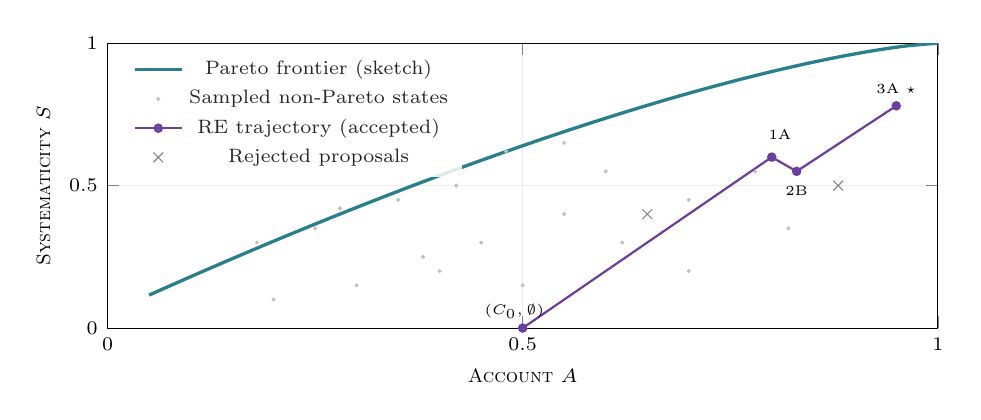
\begin{tikzpicture}
    \begin{axis}[
      width=\linewidth, height=5.2cm,
      xlabel={\textsc{Account} $A$}, ylabel={\textsc{Systematicity} $S$},
      xmin=0, xmax=1, ymin=0, ymax=1,
      xtick={0, 0.5, 1.0}, ytick={0, 0.5, 1.0},
      tick label style={font=\scriptsize}, label style={font=\scriptsize},
      grid=both, grid style={gray!15},
      legend style={font=\scriptsize, at={(0.02,0.98)}, anchor=north west, draw=none, fill=white, fill opacity=0.85},
    ]
      % Pareto frontier curve
      \addplot[epi, very thick, smooth, domain=0.05:1] {1 - 0.95*(1-x)^1.4};
      \addlegendentry{Pareto frontier (sketch)}
      % Off-frontier dominated cloud
      \addplot[only marks, mark=*, mark size=0.5pt, gray!50] coordinates {
        (0.20, 0.10) (0.30, 0.15) (0.40, 0.20) (0.18, 0.30) (0.25, 0.35)
        (0.45, 0.30) (0.50, 0.15) (0.55, 0.40) (0.62, 0.30) (0.70, 0.45)
        (0.35, 0.45) (0.42, 0.50) (0.28, 0.42) (0.60, 0.55) (0.78, 0.55)
        (0.82, 0.35) (0.55, 0.65) (0.70, 0.20) (0.48, 0.62) (0.38, 0.25)
      };
      \addlegendentry{Sampled non-Pareto states}
      % RE trajectory (accepted)
      \addplot[re, thick, mark=*, mark size=1.3pt] coordinates {
        (0.50, 0.00) (0.80, 0.60) (0.83, 0.55) (0.95, 0.78)
      };
      \addlegendentry{RE trajectory (accepted)}
      % rejected proposals (annotated)
      \addplot[only marks, mark=x, mark size=2.5pt, mcmc] coordinates {
        (0.65, 0.40) (0.88, 0.50)
      };
      \addlegendentry{Rejected proposals}
      % step labels
      \node[font=\tiny] at (axis cs:0.49, 0.06) {$(C_0, \emptyset)$};
      \node[font=\tiny] at (axis cs:0.81, 0.68) {1A};
      \node[font=\tiny] at (axis cs:0.83, 0.48) {2B};
      \node[font=\tiny] at (axis cs:0.95, 0.84) {3A $\star$};
    \end{axis}
  \end{tikzpicture}
  \captionof{figure}{\small \textbf{Epistemic Pareto frontier.} Projection onto
    $(A, S)$ with $F \approx 1$. The RE run climbs through three accepted moves and
    rejects two dominated proposals (grey $\times$). The starred final state
    sits at the frontier --- a global trade-off optimum no other reachable state
    dominates.}
  \label{fig:epi-frontier}
\end{Figure}

\begin{Figure}
  \centering
  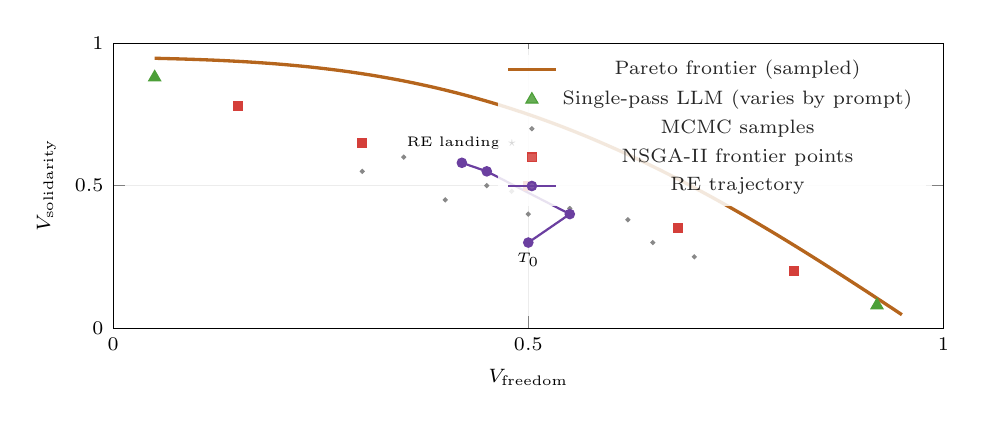
\begin{tikzpicture}
    \begin{axis}[
      width=\linewidth, height=5.2cm,
      xlabel={$V_{\text{freedom}}$}, ylabel={$V_{\text{solidarity}}$},
      xmin=0, xmax=1, ymin=0, ymax=1,
      xtick={0, 0.5, 1.0}, ytick={0, 0.5, 1.0},
      tick label style={font=\scriptsize}, label style={font=\scriptsize},
      grid=both, grid style={gray!15},
      legend style={font=\scriptsize, at={(0.98,0.98)}, anchor=north east, draw=none, fill=white, fill opacity=0.85},
    ]
      % a "frontier" of dominant mixed positions (a curve from corner to corner)
      \addplot[val, very thick, smooth, domain=0.05:0.95]
        {0.95 - x + 0.3*sin(deg(3.1416*x))};
      \addlegendentry{Pareto frontier (sampled)}
      % corner-y theories (utility-dominated, Kant-dominated)
      \addplot[only marks, mark=triangle*, mark size=2.5pt, onepass] coordinates {
        (0.92, 0.08) (0.05, 0.88)
      };
      \addlegendentry{Single-pass LLM (varies by prompt)}
      % MCMC samples
      \addplot[only marks, mark=*, mark size=0.7pt, mcmc] coordinates {
        (0.50, 0.40) (0.65, 0.30) (0.45, 0.50) (0.30, 0.55) (0.70, 0.25)
        (0.40, 0.45) (0.55, 0.42) (0.62, 0.38) (0.35, 0.60) (0.48, 0.48)
      };
      \addlegendentry{MCMC samples}
      % NSGA-II frontier points
      \addplot[only marks, mark=square*, mark size=1.6pt, nsga] coordinates {
        (0.15, 0.78) (0.30, 0.65) (0.50, 0.50) (0.68, 0.35) (0.82, 0.20)
      };
      \addlegendentry{NSGA-II frontier points}
      % RE trajectory and landing
      \addplot[re, thick, mark=*, mark size=1.5pt] coordinates {
        (0.50, 0.30) (0.55, 0.40) (0.45, 0.55) (0.42, 0.58)
      };
      \addlegendentry{RE trajectory}
      \node[font=\tiny] at (axis cs:0.50, 0.24) {$T_0$};
      \node[font=\tiny] at (axis cs:0.42, 0.65) {RE landing $\star$};
    \end{axis}
  \end{tikzpicture}
  \captionof{figure}{\small \textbf{Ethical-value Pareto frontier.} Projection of
    $V(T)$ onto $(V_{\text{freedom}}, V_{\text{solidarity}})$. Single-pass LLM
    judgment collapses to corners depending on prompt. NSGA-II traces the
    frontier. RE lands at an interior frontier point --- a defensibly mixed
    normative profile.}
  \label{fig:val-frontier}
\end{Figure}

\section{Hypotheses}

We propose two empirically testable hypotheses about reflective equilibrium.

\paragraph{H1 (Interior-bias).} RE lands on the \emph{interior} (mixed) region
of the ethical-value Pareto frontier $\Pi_V$ more reliably than do non-%
equilibrium baselines. The alternation between commitment and principle
revision penalises both under-coverage and over-specialisation, biasing the
trajectory toward defensible value mixes rather than monomaniacal corners.
H1 articulates what we mean by good moral reasoning in this framework.

\paragraph{H2 (Systematicity-driven value bias).} The systematicity desideratum
biases RE toward values that admit compact principle-level statement
(\textsc{welfare}, \textsc{justice}) and away from those that resist it
(\textsc{solidarity}, \textsc{dignity}). If confirmed, this is a substantive
philosophical finding: epistemic coherence preferences silently shape the
values a moral reasoner ends up endorsing.

\section{Methodology sketch}\label{sec:methods}

\paragraph{Data.} We use MoReBench \citep{morebench2025} and in particular the
MoReBench-Theory subset (150 scenarios with explicit framework labels), which
gives us framework-tagged dilemmas without doing the tagging ourselves.

\paragraph{Pipeline.} The construction of the data resource is a careful
multi-stage process; the resource itself is what makes the downstream traversal
comparisons cleanly interpretable.
\begin{enumerate}[leftmargin=*, itemsep=2pt, label=(\roman*)]
  \item \emph{Generation.} For each of $\sim$10 dilemmas, LLM-generate a
    commitment pool ($\sim$30 candidates) and a principle pool ($\sim$20
    candidates: half value-archetypal, half bottom-up from the commitments).
  \item \emph{Curation.} This is the load-bearing stage. We fuse near-duplicate
    principles, drop principles with weak independent credibility, and score
    each surviving principle on quality dimensions independent of the
    equilibration loop --- per-principle systematicity (how general /
    unifying is this principle taken on its own?), specificity, and
    domain-appropriateness. The curated pool is then double-checked by
    philosophers, both to verify the value tagging in (iii) and to catch
    principles whose moral content the LLM has misread. The intent is that the
    final pool is a high-quality \emph{moral resource} in its own right ---
    something a researcher could reuse independently of any particular
    traversal method.
  \item \emph{Value tagging.} LLM-tag each surviving principle with a
    value-loading vector $\boldsymbol{v}(p) \in [0, 1]^K$ over the five values;
    MoReBench-Theory's framework labels serve as calibration anchors
    (utilitarian-framework labels seed welfare loadings, Kantian-framework
    labels seed dignity / justice, etc.). Philosopher review confirms loadings.
  \item \emph{Dialectical structure.} Pre-compute $\rho: \mathcal{P} \times
    \mathcal{S} \to \{\text{entails}, \text{contradicts}, \text{silent}\}$
    for every principle-commitment pair as a one-time batch.
\end{enumerate}
The output of this pipeline is a \emph{curated, mathematically well-defined
moral space} $\tau = \langle \mathcal{S}, \mathcal{P}, \rho\rangle$ together
with the value-loading map $\boldsymbol{v}$, on which any traversal method
can be evaluated.

\paragraph{Traversals.} The primary object of study is symbolic RE on the
curated pool. To put its behaviour in context we run a small set of comparison
traversals on the same pool: a single-pass LLM judgment baseline (with no
equilibration), and a NSGA-II reference that estimates $\Pi_V$ and $\Pi_E$
without committing to any particular reasoning strategy. Each yields a
distribution of $(A, S, F, V_1, \dots, V_K)$ points.

\paragraph{Analysis.} Locate RE's landing distribution on $\Pi_E$ and $\Pi_V$
relative to NSGA-II and the single-pass baseline. Test H1 (interior bias) by
Mann-Whitney displacement against single-pass on $\Pi_V$; test H2
(systematicity-driven value bias) by directional displacement of RE landings
relative to NSGA-II frontier points at matched epistemic cost.

\section{Discussion}

The framing answers two long-standing complaints about RE without rejecting them.
\emph{Pluralism} (de Maagt, Singer) is real but not relativism: the frontier picks
out a proper subset of all positions, and being on it is a substantive constraint.
\emph{Conservatism} (Brandt, Kelly--McGrath) is real but not damning: it shows up
as a systematic landing-region offset toward $F = 1$, which a method comparison can
quantify rather than dismiss. And the underlying philosophical question --- what
\emph{is} good moral reasoning? --- becomes empirically tractable as a property of
traversal strategies relative to a measurable solution topology.

The contribution we are aiming at is not another moral-reasoning benchmark, nor
another RE-vs-critics dialectic. It is a measurement instrument:
value-trajectory plots and Pareto-region analyses that any LLM-based or symbolic
moral reasoning system can be characterised against.

\bibliographystyle{plainnat}
\bibliography{references}

\end{multicols}

\end{document}
